\documentclass{article}

\usepackage[utf8]{inputenc}
\usepackage[T1]{fontenc}
\usepackage[french]{babel}
\usepackage{amsmath, amssymb}
\usepackage{color}
\usepackage{ifthen}
%\usepackage{showframe}

\usepackage{graphicx}
\graphicspath{{graphics/}}

\usepackage{geometry}
\geometry{
    a4paper,
    total={150mm,230mm},
}

\usepackage{listings}
\lstset{
    language=C++,
    literate=
        {à}{{\`a}}1
        {é}{{\'e}}1
        {è}{{\`e}}1
        {ê}{{\^e}}1
        {ô}{{\^o}}1
        {ç}{{\c{c}}}1,
    basicstyle=\small,
    identifierstyle=\ttfamily,
    keywordstyle=\color[rgb]{0, 0, 1},
    commentstyle=\color[rgb]{0.133, 0.545, 0.133},
    stringstyle=\color[rgb]{0.627, 0.126, 0.941},
}

\usepackage{hyperref}
\hypersetup{
    colorlinks=true,
    urlcolor=blue
}

\newcommand{\diff}[1]{\mathop{\mathrm{d}#1}}
\newcommand{\esp}[1]{\mathbb{E}[#1]}
\newcommand{\var}[1]{\mathrm{Var}(#1)}
\newcommand{\link}[2]{\href{#1}{\color[rgb]{0, 0, 1}#2}}

\newcounter{questionsCounter}
\newcounter{pointsCounter}
\newcommand{\question}[1]{%
    \addtocounter{questionsCounter}{1}%
    \addtocounter{pointsCounter}{#1}%
    \vspace{-8pt}\paragraph{Q\arabic{questionsCounter} (#1 pt\protect\ifthenelse{#1 = 1}{}{s})}%
}

% Comment the \renewcommand to show the correction notes
\newcommand{\hidden}[1]{{\color[rgb]{1, 0, 0}#1}}
\renewcommand{\hidden}[1]{}


\title{EIING3D1 - TP Échantillonnage adaptatif\hidden{\\Version stylo rouge}}
\author{francois.desrichard@irit.fr}
\date{}


\begin{document}

\maketitle


\section{Introduction}
On a vu en cours que l'irradiance $I_j$ reçue sur un pixel $j$ du plan caméra peut s'exprimer comme une intégrale sur l'espace des chemins $\Omega$ :%
%
\begin{equation*}
    I_j = \int_\Omega f(\bar{p}) \diff{\mu}(\bar{p})
\end{equation*}

Afin d'estimer la valeur de $I_j$, les algorithmes de rendu basés sur l'intégration de Monte-Carlo génèrent aléatoirement des échantillons, des chemins lumineux $\bar{p}$ reliant une source au point $j$.
Le logiciel pbrt-v3 propose un ensemble d'intégrateurs implémentant cette estimation dans une méthode \texttt{Render} (\link{http://www.pbr-book.org/3ed-2018/Introduction/pbrt_System_Overview.html\#Integrator}{documentation en ligne}).
Pour le Path Tracing, \texttt{Render} prend la forme suivante :%
%
\begin{lstlisting}
void Render(const Scene &scene) {
    ParallelFor2D([&](Point2i tile) {
        for (Point2i pixel : tileBounds) {
            do { /* Générer un chemin aléatoire */ }
            while (tileSampler->StartNextSample());
\end{lstlisting}

\begin{figure*}
    \centering
    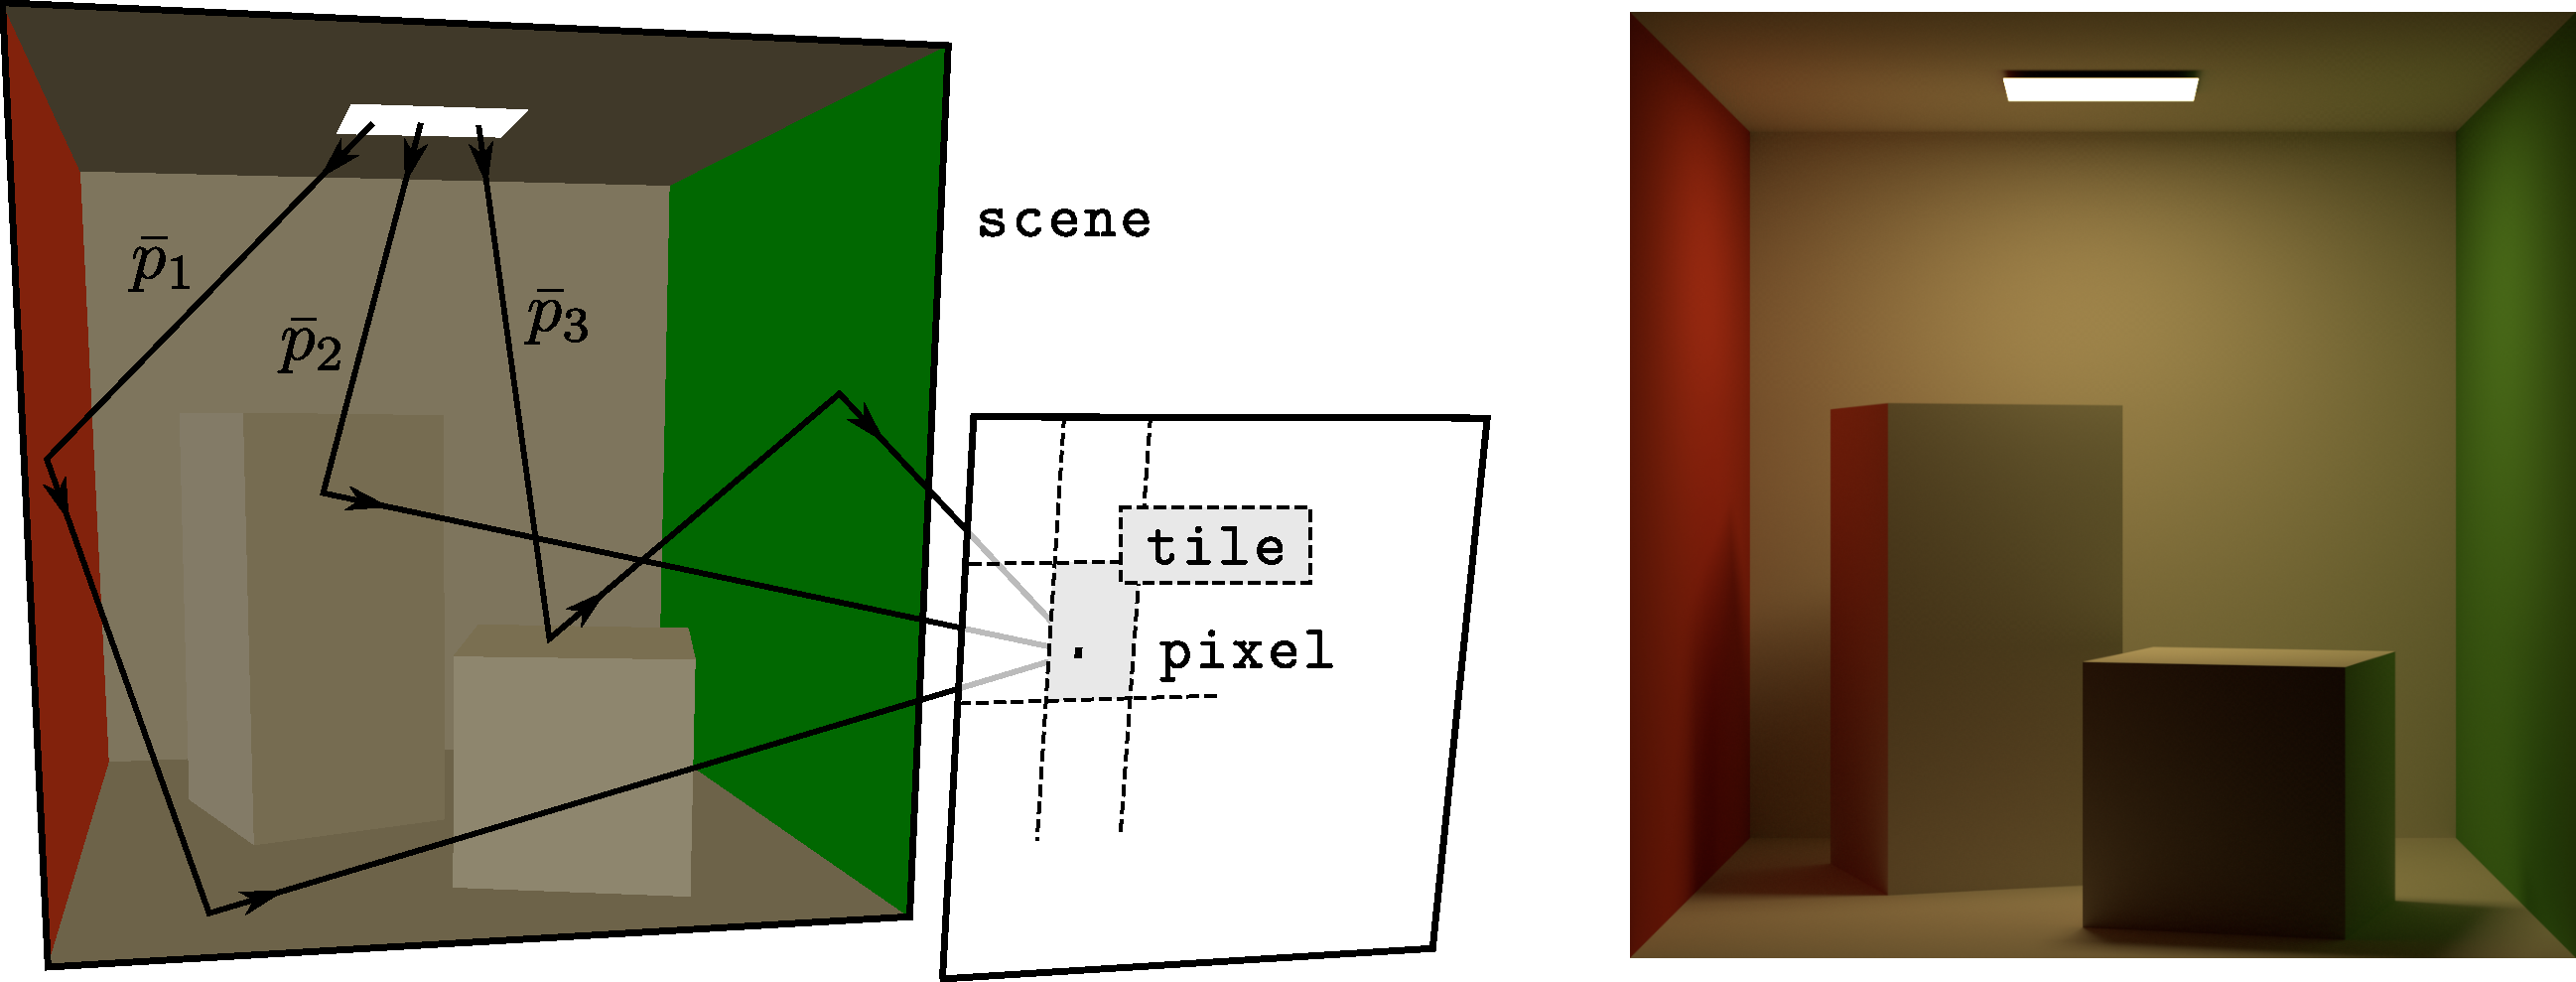
\includegraphics[width=\linewidth]{render_loop}
\end{figure*}

L'image est découpée en tuiles traitées en parallèle, et les pixels de chaque tuile sont parcourus séquentiellement.
En chacun, \texttt{tileSampler} génère $N$ séquences de nombres aléatoires afin de construire $N$ chemins lumineux ; l'intégrateur approche $I_j$ en moyennant leurs contributions.
On appelle $X$ la variable aléatoire (VA) représentant la contribution lumineuse d'un chemin et $(X_1, \ldots\, X_N)$ des VA i.i.d. selon la même loi que $X$ qui représentent les différents échantillons.
La moyenne empirique $\overline{X}_N$ est un estimateur non biaisé de l'espérance de $X$ :%
%
\begin{equation*}
    \overline{X}_N = \frac{1}{N} \sum_{i = 1}^{N} X_i
    \:\;\xrightarrow{p}\:\: \esp{X} = I_j
\end{equation*}

Le nombre d'échantillons $N$ ne dépend pas du pixel : on parle d'échantillonnage uniforme.
Cependant la complexité du transport lumineux varie localement, et la vitesse de convergence de l'estimateur aussi ; nous allons donc adapter l'échantillonnage pour améliorer le rendu.


\section{Estimation des statistiques par pixel}

Un intégrateur \texttt{VolPathAdaptive} a été ajouté à pbrt ; sa méthode \texttt{Render} sépare le rendu en lots \emph{(batches)} et tire un nombre arbitraire d'échantillons :%
%
\begin{lstlisting}
void Render(const Scene &scene) {
    for (int i = 0; stats.StartNextBatch(i); ++i) {
        ParallelFor2D([&](Point2i tile) {
            for (Point2i pixel : tileBounds) {
                stats.SamplingLoop(pixel, [&]() {
                    // stats contrôle la boucle de rendu
                    tileSampler->StartNextSample();
                    return L;
                });
\end{lstlisting}

Pour l'instant, l'intégrateur fonctionne comme \texttt{VolPathIntegrator} : il traite un seul lot à $N_j = N$ fixé.
L'objet \texttt{stats} intercepte la contribution lumineuse de chaque échantillon afin d'estimer des statistiques sur le rendu de chaque pixel.

\question{1} Le calcul de la moyenne $\bar{x}$ et du moment d'ordre 2 est basé sur une suite de valeurs obtenues au fur et à mesure du rendu.
Pour éviter de les stocker, nous aurons recours à l'algorithme de Welford (\link{https://en.wikipedia.org/wiki/Algorithms_for_calculating_variance\#Welford's_online_algorithm}{Wikipédia}) ; l'implémenter dans \texttt{UpdateStats}.

\question{2} Utiliser l'estimateur non biaisé de la variance dans la fonction \texttt{Variance} ; nous le noterons $S^2$.
Commenter un rendu : quelles sont les zones de faible / forte variance ? Pourquoi ?

\hidden{%
Zones de forte variance : frontière d'une source lumineuse, surfaces glossy - spéculaires, caustiques, frontières d'ombre, géométrie intriquée...
Zones de faible variance : surfaces diffuses, trajets directs vers une source lumineuse...
Toute explication judicieuse est bonne à prendre.
}


\section{Définition et analyse de l'erreur}

L'erreur standard est définie à partir de $s^2$, la variance estimée par $S^2$ :%
%
\begin{equation*}
    \sigma_{\bar{x}} = \sqrt\frac{s^2}{N}
\end{equation*}

C'est une erreur absolue : son unité est celle de la grandeur calculée.
Au contraire l'erreur relative s'exprime en pourcentage :%
%
\begin{equation*}
    RSE_{\bar{x}} = \frac{\sigma_{\bar{x}}}{\bar{x}}
\end{equation*}

\question{1} Quel est le comportement asymptotique de l'erreur lorsque $N \rightarrow +\infty$ ?

\hidden{%
$o(1/\sqrt N)$.
Erreur standard ou relative ? Pareil.
}

\question{2} Compléter \texttt{Error} avec ces deux formules.
Que devient l'erreur relative quand la moyenne tend vers zéro ? Proposer un terme correctif.

\hidden{%
Bien sûr il y a divergence, c'est la deuxième partie de la question qui est intéressante.
Mitsuba utilise par exemple un max entre la moyenne et la luminance moyenne de l'image * 0.01.
D'autres expériences sont possibles, par exemple en lissant la singularité avec une fonction du type $\sqrt{\mathrm{cst}^2 + \bar{x}^2}$ au dénominateur.
Toute bonne réflexion est valorisée, en faisant attention quand même à l'homogénéité des quantités proposées.
}

\question{1} Comparer les résultats des deux versions sur des zones choisies.

\hidden{%
L'important est de remarquer que l'erreur standard explose à certains endroits de l'image (source de lumière après un rebond, etc.) et que l'on ne peut pas toujours utiliser un seuil global sur l'image avec cette définition.
Au contraire, l'erreur relative est sans unité.
}


\section{Contrôle adaptatif de la qualité}

Par défaut, l'intégrateur est en mode \texttt{normal} et tire \texttt{maxSamples} échantillons.
Nous allons ajouter un mode \texttt{error} qui tire un nombre d'échantillons variable entre \texttt{minSamples} et \texttt{maxSamples} en fonction de l'erreur commise.

\question{2} Ajouter une clause dans \texttt{SamplingLoop} pour séparer le rendu du pixel en deux étapes : dans la première \emph{(bootstrap)}, on tire \texttt{minSamples} échantillons ; dans la seconde \emph{(adaptive)}, on tire des échantillons jusqu'à satisfaire le critère d'arrêt \texttt{StopCriterion}.

\hidden{%
Faire attention à ce que le nombre maximal de samples soit toujours respecté.
Pour passer d'un \texttt{Spectrum} à un \texttt{Float}, plusieurs possibilités.
Couramment, on préfèrera utiliser la luminance \texttt{y} pour avoir une heuristique proche de la perception humaine.
L'utilisation de \texttt{MaxComponentValue} est aussi possible mais très pessimiste en pratique.
Valoriser toute discussion intéressante.
}

\question{2} Modifier la fonction \texttt{Sampling} pour renvoyer une valeur entre $0$ et $1$ indiquant la proportion d'échantillons supplémentaires utilisée.
Comment évolue l'échantillonnage dans l'image en mode \texttt{error} ? Que dire de l'erreur ?

\hidden{%
Il faut amener la réflexion sur la dualité entre échantillonnage et erreur : on passe d'un échantillonnage uniforme / erreur variable sur l'image à un échantillonnage variable / erreur "uniformisée" car seuillée dans l'idéal.}


\section{Comparaison avec un rendu en temps fixe}

Avec le nombre d'échantillons et l'erreur de l'estimateur, la troisième grandeur à prendre en compte est le temps de calcul, ressource que l'on souhaite économiser.
Le découpage de \texttt{Render} en lots permet de contrôler le temps de rendu total avec une certaine précision.

\question{2} Ajouter à \texttt{SamplingLoop} et \texttt{StartNextBatch} le mode \texttt{time} où l'intégrateur tire un nombre fixe \texttt{batchSize} d'échantillons par pixel et par lot jusqu'à atteindre le temps maximal, sans toutefois dépasser \texttt{maxSamples}.

\hidden{%
Pour fixer \texttt{batchSize}, il faut prendre une petite valeur pour avoir une bonne précision, mais rester cohérent avec le ratio temps / échantillon ; on se fait une idée de ce ratio après avoir rendu 2 - 3 fois une scène durant le TP.
}

\question{4} Proposer et mettre en œuvre un protocole pour évaluer l'échantillonnage adaptatif.
Les scènes comprenant un sujet complexe sur fond mat fournissent généralement de bons exemples.

\hidden{%
Le protocole doit ressembler à : "Je commence par un rendu en mode \texttt{normal} avec un nombre d'échantillons suffisant pour estimer l'erreur.
J'ai bien fait attention d'exporter un EXR donc je peux pointer les zones problématiques de l'image et obtenir leur erreur relative.
Je passe en mode \texttt{error} avec un seuil adapté aux zones problématiques ; le nombre d'échantillons du mode \texttt{normal} devient par exemple le \texttt{minSamples} du mode \texttt{error}, et pour \texttt{maxSamples} je choisis 4 fois ça afin de diviser l'erreur par 2.
Je récupère le temps de rendu depuis le profiler (\texttt{Integrator/Render time} étant le plus précis) pour lancer un rendu en mode \texttt{time} de même durée.
Je compare les deux derniers rendus et je remarque que l'erreur tend à s'uniformiser et que l'image est plus belle...
}


\section{Intervalles de confiance}

On souhaiterait garantir sur nos résultats un taux de confiance $\alpha$.
On va voir que l'on peut calculer un certain $t$ qui définit un intervalle de confiance $C = [\bar{x} - t, \,\bar{x} + t]$ ; par construction, $100\alpha\%$ des intervalles estimés contiendront la véritable valeur $I_j$.
Intuitivement à fort taux de confiance, grand intervalle : on peut affirmer à $99.99\%$ avoir encadré la véritable valeur, mais par des bornes gigantesques.
Inversement à faible taux de confiance, petit intervalle : on peut fournir des estimations fines, sans garantir du tout que la vraie valeur tombe dedans...

On commence par centrer et réduire l'estimateur de la moyenne $\overline{X}_N$, ce qui définit la VA $Z_N$ :%
%
\begin{equation*}
    Z_N = \frac{\overline{X}_N - I_j}{\sqrt{\var{X}/N}}
\end{equation*}

\noindent Comme $N$ est fixé, $Z_N$ suit une distribution de Student (\link{https://en.wikipedia.org/wiki/Student\%27s_t-distribution}{Wikipédia}).
Cependant pour simplifier, nous allons utiliser le théorème central limite qui assure que lorsque $N \rightarrow +\infty$, $Z_N$ converge en loi vers $Z$ une gaussienne centrée réduite et suit donc approximativement $\mathcal{N}(0, 1)$ lorsque $N$ est assez grand.
On cherche maintenant un certain $z$ qui encadre $Z$ avec probabilité $\alpha$ :%
%
\begin{equation*}
    \mathrm{P}(-z < Z < z) = \alpha
\end{equation*}%
%
Par la relation de Chasles et la symétrie de la fonction de distribution $f_Z$ :%
%
\begin{equation*}
\begin{split}
    \mathrm{P}(-z < Z < z)\,
    = \int_{-z}^{+z} f_Z
   &= \int_{-z}^{+\infty} f_Z + \int_{+\infty}^{-\infty} f_Z + \int_{-\infty}^{+z} f_Z\\
   &= \int_{-\infty}^{+z} f_Z - \int_{-\infty}^{+\infty} f_Z + \int_{-\infty}^{+z} f_Z
    = \,2\Phi_Z(z) - 1
\end{split}
\end{equation*}%
%
où $\Phi_Z$ est la fonction de répartition de $Z$.
Pour une distribution normale $\mathcal{N}(0, 1)$ elle est appelée fonction d'erreur de Gauss ; comme elle est inversible,%
%
\begin{equation*}
    \alpha = \,2\Phi_Z(z) - 1
    \;\Leftrightarrow\;
    z = \Phi_Z^{-1}\left(\frac{1 + \alpha}{2}\right)
\end{equation*}

On connait maintenant pour $Z$ la largeur $z$ de l'intervalle en fonction du taux de confiance $\alpha$.
Pour revenir à $\overline{X}_N$ et obtenir $t$ la largeur de l'intervalle, on réinjecte la variance estimée :%
%
\begin{equation*}
    t = z\sqrt{s^2/N} = z\sigma_{\bar{x}}
\end{equation*}%
%
et on recentre enfin l'intervalle autour de $\bar{x}$ :%
%
\begin{equation*}
    C = [
        \bar{x} - z\sigma_{\bar{x}},\,
        \bar{x} + z\sigma_{\bar{x}}
    ]
\end{equation*}

En pratique $z$ est tabulé selon des valeurs courantes de $\alpha$ (\link{https://en.wikipedia.org/wiki/Confidence_interval\#Basic_steps}{Wikipédia}).
Attention, vous trouverez majoritairement une autre convention où $\alpha \rightarrow 1 - \alpha$.

\question{3} Ajouter une condition d'arrêt basée sur l'intervalle de confiance.
Une implémentation tirant parti de la bibliothèque \link{https://www.boost.org/doc/libs/1_71_0/doc/html/boost_random/reference.html\#boost_random.reference.distributions}{boost::random}, comme c'est le cas dans le logiciel \link{https://www.mitsuba-renderer.org/}{Mitsuba}, permet de laisser à l'utilisateur le libre choix de $\alpha$.

\hidden{%
En soit la première partie de la question revient à diviser le seuil d'erreur standard par $z$, donc pour avoir tous les points on attend un peu mieux.
}

\hidden{TOTAL POINTS = \arabic{pointsCounter}}

\end{document}
